\chapter[Integração]{Integração}

\section{Motivação}
Após as primeiras tentativas de rodar a aplicação com o objetivo de identificar defeitos que deveriam ser corrigidos para garantir o funcionamento do MVP do Agromart, foi notado um gargalo no processo de execução da aplicação para testes e desenvolvimento local. Tal situação ocorreu devido às características do projeto, que envolvem a execução de três aplicações: a API Dicionário, o Backend e o Aplicativo Mobile.

Desse modo, a primeira motivação para ter esses servidores rodando em ambientes reais foi facilitar o processo de teste e desenvolvimento do sistema, para que fosse necessário rodar localmente apenas o Aplicativo Mobile, apontando para os ambientes da nuvem.

A segunda motivação foi a necessidade de ambientes reais rodando, acessíveis via HTTPS, para que fosse também gerada uma versão de produção do aplicativo e que pudesse ser devidamente publicada na Google Play Store, uma vez que os aplicativos publicados passam por revisão manual. Sendo assim o aplicativo só poderia ser aprovado na loja se estivesse se comunicando com servidores reais e persistindo dados corretamente.

\section{Serviço Escolhido para deploy dos servidores}
O Amazon EC2 (Elastic Compute Cloud) é um serviço de computação em nuvem da AWS (Amazon Web Services) que permite aos usuários criar máquinas virtuais em nuvem com diferentes configurações de CPU, memória, armazenamento e rede. Essas instâncias podem rodar sistemas operacionais, aplicativos e outros serviços, permitindo que você execute cargas de trabalho como se estivesse utilizando servidores físicos, mas com a flexibilidade e escalabilidade da nuvem.Essas configurações podem ser facilmente manipuladas de acordo com a necessidade do usuário.

A principal razão para a escolha da EC2 na realização do deploy dos servidores foi a flexibilidade que o serviço oferece para modificar os recursos da instância alocada. Sem saber inicialmente quanto recurso seria necessário para o bom funcionamento do Agromart, a escolha de uma opção que permitisse a fácil manipulação dos recursos computacionais foi fundamental.

\section{Processo de deploy do servidores}
Levando em conta as necessidades listadas, foi alocada uma instância EC2 na AWS para disponibilizar a API Dicionário e o Backend do Agromart. A instância EC2 selecionada possui as seguintes características: tipo de instância t3.medium, com 2 vCPUs, 4 GB de memória RAM, e um volume de armazenamento de 30 GB em um SSD como visto na Fig. \ref{ec2}. O sistema operacional escolhido foi o Linux, e a instância foi alocada na região da AWS da Virgínia do Norte (us-east-1).

Adicionalmente, também foram criados snapshots do volume para recuperar o estado dos servidores em caso de falha. A configuração foi realizada com o objetivo de balancear adequadamente o custo e o desempenho.

\begin{figure}[h]
        \centering
        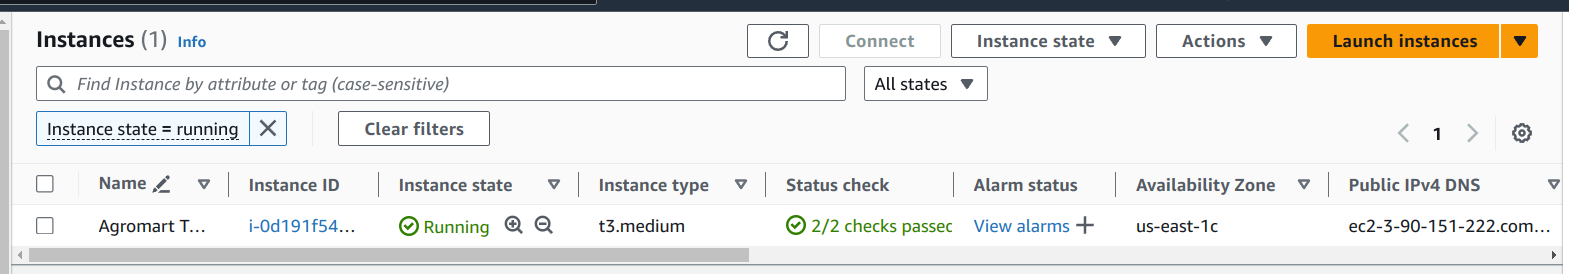
\includegraphics[keepaspectratio=true,scale=0.3]{figuras/ec2_agromart.png}
        \caption{Imagem da EC2 do Agromart}
        \label{ec2}
\end{figure}

\subsection{Preparação do Banco de Dados}
Para a preparação do banco de dados, foi utilizado o SGBD PostgreSQL. A imagem oficial do PostgreSQL foi usada para criar o banco de dados em um ambiente Docker. Essa abordagem foi escolhida por ser uma forma rápida de instalar e rodar o banco de dados no servidor.

\subsection{Aquisição de Domínio}
Um domínio foi essencial para conseguirmos um certificado SSL válido, que por sua vez é necessário para que possamos habilitar o HTTPS em nosso servidores. O domínio foi comprado através da plataforma Hostinger, e seu endereço é agromarttcc.shop, por um prazo de 1 ano, conforme apresentado na Fig. \ref{dominio}. 

\begin{figure}[h]
	\centering
	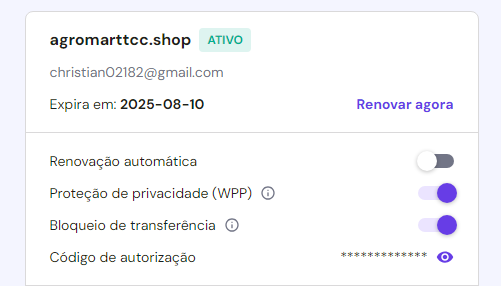
\includegraphics[keepaspectratio=true,scale=0.35]{figuras/dominio.png}
	\caption{Visualização do domínio na plataforma Hostinger}
	\label{dominio}
\end{figure}

\subsection{Configuração de HTTPS, domínio e certificado}
HTTPS (Hypertext Transfer Protocol Secure) é uma versão segura do protocolo HTTP, usado para a comunicação entre navegadores web e servidores. A principal diferença é que o HTTPS criptografa os dados enviados e recebidos, garantindo maior segurança das informações transmitidas.

No caso do Agromart, disponibilizar nossos servidores através de HTTPS é extremamente necessário, pois chamadas puramente HTTP não são permitidas em aplicativos publicados na Google Play Store.

O Nginx é uma ferramenta para servidores web poderosa e muito utilizada, no contexto do Agromart, utilizamos o Nginx como Proxy Reverso dos nossos servidores (CSAs implantadas e API dicionário). Dessa forma todas chamadas feitas aos nossos servidores passam primeiro pelo Nginx, que encaminha para o servidor correto. O proxy reverso com Nginx também permitiu a implementação de certificados SSL que era necessário para o protocolo HTTPS.

 O certificado SSL necessário para habilitar o HTTPS foi obtido gratuitamente através da ferramenta Certbot, que nos proveu um certificado para o domínio agromarttc.shop.

 Com todas essas configurações feitas, a única coisa restante foi apontar o nosso domínio para o IP público da nossa máquina virtual onde os servidores estavam rodando, esse processo foi feito pelo painel da Hostinger.

\section{Processo de deploy do Aplicativo na Google Play Store}

\subsection{Conta no Expo e EAS}
O Aplicativo do Agromart foi criado utilizando uma ferramenta chamda Expo. O Expo é uma plataforma de desenvolvimento de aplicativos com React Native, que foi a tecnologia escolhida para o aplicativo em sua idealização.

o EAS (Expo Application Services) é um conjunto de ferramentas para deploy de aplicativos que utilizam o Expo. Utilizamos o serviço EAS Build, que permite compilar e gerar buils para Android na núvem, sem necessidade de instalação de ferramentas para compilação localmente.

Para isso, foi criada uma conta do Expo específica para esse projeto de conclusão de curso, para build da versão de produção que foi sumetida à Google Play Store. Na figura \ref{expo}, podemos ver a conta no Expo e algumas das builds de produção geradas.

\begin{figure}[h]
	\centering
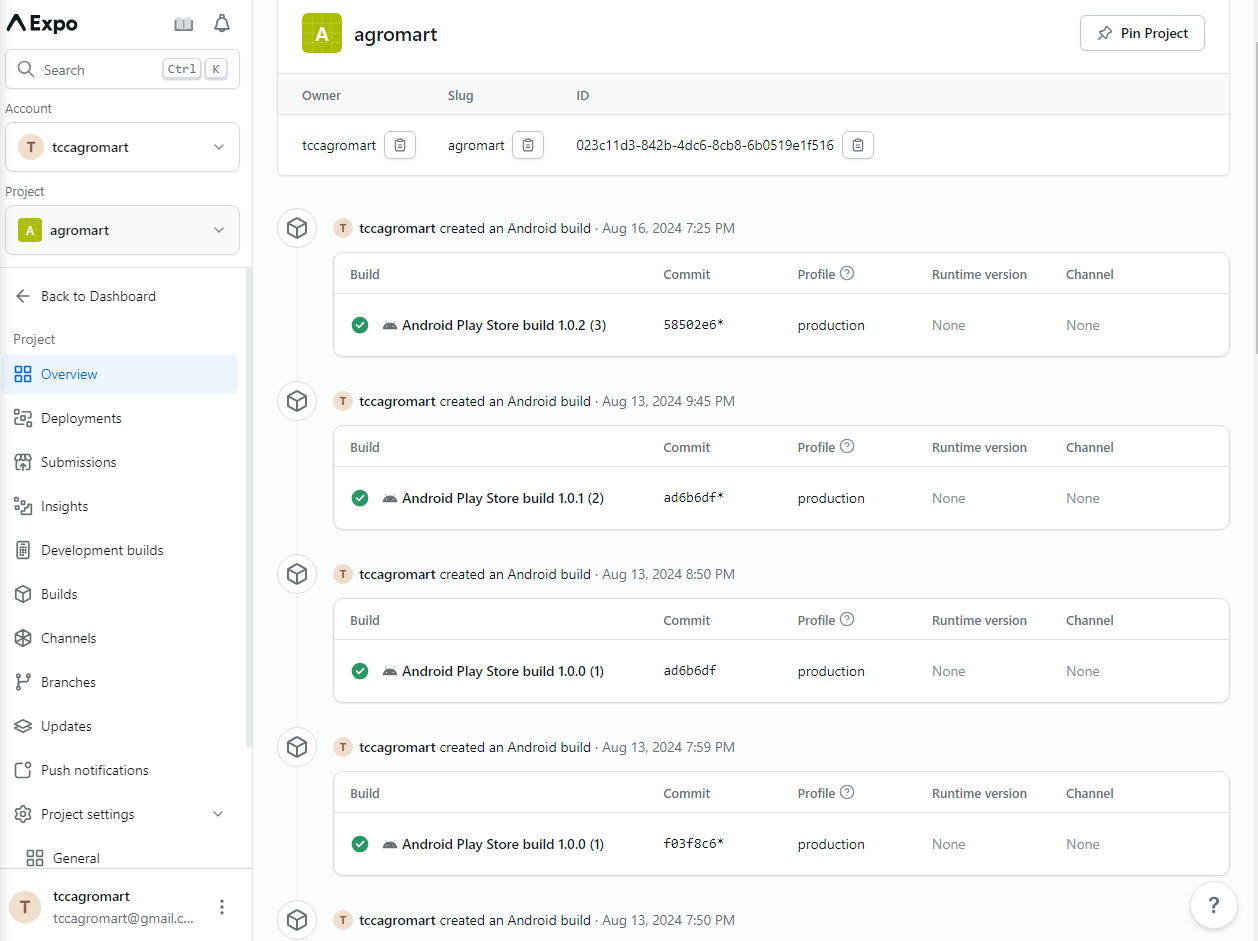
\includegraphics[keepaspectratio=true,scale=0.35]{figuras/expo.png}
	\caption{Painel da conta Expo com Builds realizadas}
	\label{expo}
\end{figure}

\subsection{Geração de Builds de produção}

Uma build de produção é uma versão de um software que está pronta para ser lançada e usada pelos usuários finais. Após a correção de diversos defeitos, pudemos enfim concluir que tinhamos atingindo já um MVP do Agromart, e gerar nossa primeira build de produção.

Após isso, executamos o comando \texttt{eas build --profile production --platform android.} Esse comando dispara a compilação em núvem, gerando um arquivo .aab, que é o o arquivo que devemos submeter à Play Store.

\subsection{Configuração do Aplicativo na Google Play Store e Publicação}
